\documentclass[conference]{IEEEtran}
\IEEEoverridecommandlockouts
% The preceding line is only needed to identify funding in the first footnote. If that is unneeded, please comment it out.
\usepackage{cite}
\usepackage{amsmath,amssymb,amsfonts}
\usepackage{algorithmic}
\usepackage{minted}
\usepackage{graphicx}
\usepackage{textcomp}
%\usepackage{xcolor}
\usepackage[table,xcdraw]{xcolor}
\def\BibTeX{{\rm B\kern-.05em{\sc i\kern-.025em b}\kern-.08em
    T\kern-.1667em\lower.7ex\hbox{E}\kern-.125emX}}



\graphicspath{ {./graphs/} }
\usemintedstyle{borland}
\usepackage{hyperref}
\hypersetup{
    colorlinks=true,
    linkcolor=black,
    urlcolor=black
}
\date{\today}

\begin{document}


\title{Benchmarking freeRTOS on PC \& Raspberry Pi}

\author{
    \IEEEauthorblockN{Stylianos Tsagkarakis}
    \IEEEauthorblockA{\textit{MIEEC - FEUP} \\
    \url{up201911231@fe.up.pt}}
\and
    \IEEEauthorblockN{Alena Tesařová}
    \IEEEauthorblockA{\textit{MIEEC - FEUP} \\
    \url{up201911219@fe.up.pt}}
}

\maketitle


\begin{abstract}
Project developed within the scope of the Embedded Systems curricular unit, with the objective of benchmarking FreeRTOS on the platform or Raspberry Pi 2B and Linux Kernel.
% There are many kind of Implementation on Real-time operating Systems (RTOS) can be found at the present time. The correctness of an RTOS depends not only on the logical result of the computation, but also on the correctness of temporal parameters of the task set used in the system. So, it becomes necessary to measure the response time of real-time mechanisms to predict the performance of RTOS. In recent years, several approaches have been implemented for benchmarking the real-time parameters. In this report we review some benchmarking techniques for measuring the real-time parameters of RTOS. We discuss the need of measuring real-time parameters and provide a helpful guide on benchmarking real-time operating systems for future work.

\end{abstract}

\begin{IEEEkeywords}
Real-Time Systems, RTOS, Performance
\end{IEEEkeywords}

\section{Introduction}

An operating system is said to be real time when it
schedules the execution of programs in time, handles system
resources and gives a reliable basis for the development of
software code. \cite{b1}
% Any RTOS basically has characteristics like
% Multitasking and Preemptibility, Task Priority, Priority
% Inheritance, Short Latencies (Task switching latency
% Interrupt latency, Interrupt dispatch latency), Reliable
% and Sufficient Inter Task Communication Mechanisms,
% Control of Memory Management.

Timing is the most important factor in any real time
applications. In real-time systems, all real-time tasks are differentiated
based on their timing, such as sporadic, response time,
deadline etc. Real time systems are classified in to two
types’ hard real-time systems and soft real time systems.
Hard real time system means it should complete the task
with in the deadline period otherwise its computation is
useless. The damages caused by the hard real time systems
are irreparable. 
% The system builder’s should responsible to
% choose an operating system that can support and schedule
% these jobs with respect to their timing criteria so that no
% deadline will be missed. 
Soft real time systems require
performance assurances from the operating system.

\section{Hardware}

\subsection{Specifications of hardware used for Benchmarks}

\begin{itemize}
    \item Raspberry Pi Raspberry Pi 2 Model B (ARM Cortex-A7 900MHz), 1GB RAM 
    %as seen in Figure \ref{demo}.
    \item Ubuntu 18.04, Linux Kernel 5.3.0-53-generic, Intel(R) Core(TM) i7-6500U CPU @ 2.50GHz, 12GB RAM (1 core \& 2 threads were used)
\end{itemize}

% \begin{figure}[htbp]
%     \centerline{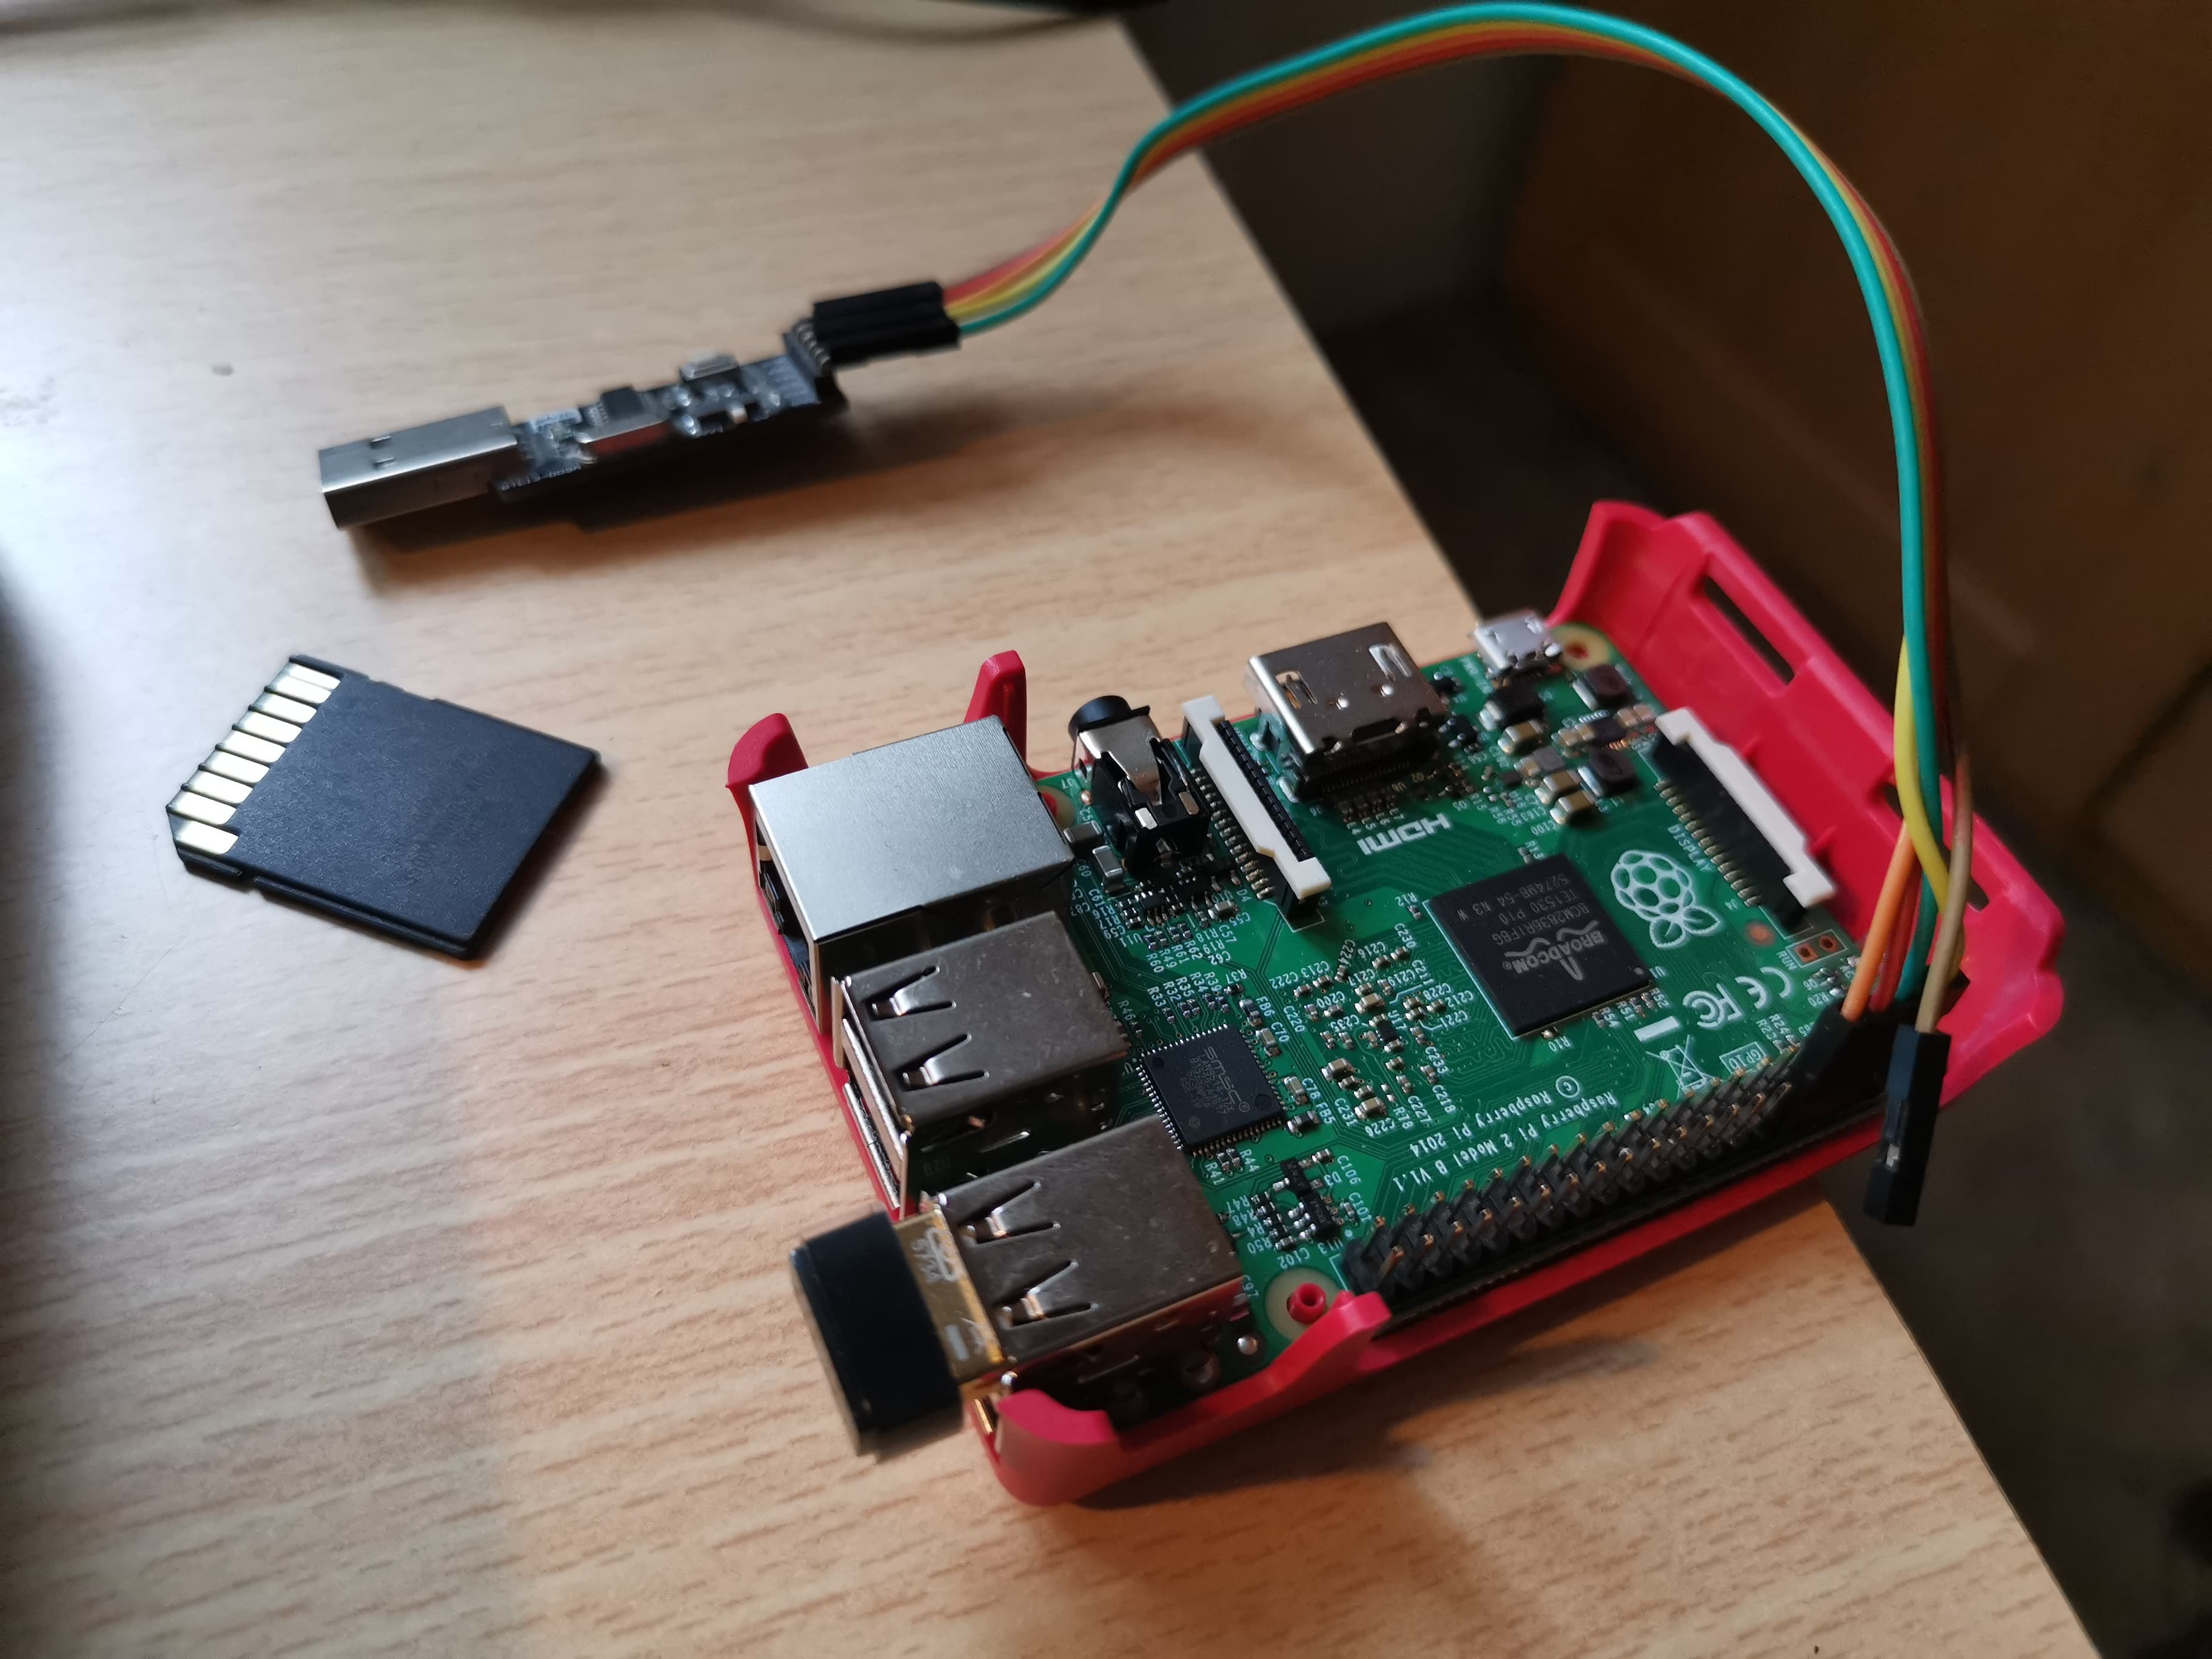
\includegraphics[width=0.7\columnwidth]{demo.jpg}}
%     \caption{RPi 2B Hardware Setup.}
%     \label{demo}
% \end{figure}

\section{Evaluating Resources}

By reading documentation \cite{b6}, related previous work \cite{b4} we managed to generate the array below stating characteristics of freeRTOS:

\begin{table}[htbp]
    \begin{center}
        \begin{tabular}{|l|l|l|}
        \hline
        \textbf{Multitasking}  & \textbf{RR Scheduling} & \textbf{Priority} \\ \hline
            \begin{tabular}[c]{@{}l@{}}Preemptive or\\ Cooperative\end{tabular} & Yes                          & Unlimited                                     \\ \hline
        \textbf{\# Tasks}                                                    & \textbf{Compilers Supported} & \textbf{Kernel size (KB)}                                        \\ \hline
        Unlimited                                                           & IAR/Keil/gcc                 & \begin{tabular}[c]{@{}l@{}}ROM: 2.7-3.6\\ RAM: 0.19\end{tabular} \\ \hline
        \end{tabular}
    \end{center}
\end{table}

In order to complete this project we used the scheduler freeRTOS has already implemented. This scheduler works based on this policy: \textbf{Highest priority task is granted CPU time.} If multiple tasks have equal priority, it uses round-robin scheduling among them. Lower priority tasks must wait.
It is important that high priority tasks don't execute 100\% of the time, because lower priority tasks would never get CPU time (starvation problem). It's a fundamental problem of real-time programming.

\vspace{-2.30mm}
\section{Testing}

\subsection{Timing}
To count the desired value two timers were used that counted the time based on this assembly instruction: 

\begin{minted}[]{c}
asm volatile("mrc p15,0,\%0,c9,c13,0":"=r"(cc))
\end{minted}

\noindent and we could get a low level timer using the processor clock speed. By using software times to count values of nanosecond accuracy we would not have the same results.

\subsection{Tests}
In this section we will briefly describe the tests and obtained results. In each test we measured the the time of one specific operation for at least 500 iterations to get better average value. Then, we run the test more times to really get reliable results. We performed 4 types of tests regarding:
\begin{itemize}
    \item Cooperative context switch (Round Robin)
    \item Message Queue
    \item Semaphores
    \item Mutexes
\end{itemize}
\vspace{-2.30mm}

\section{Results}

In cooperative scheduling we had 2 tasks with the same priority that were switching the context in round robin fashion. As we can see from the Table \ref{tab:results}, we got a median time 168 ns -- so we can use it as a starting time for other tests using context switch. However, it is not the best time we got. The lowest time we got for Receive test (137 ns) -- that is the time it takes to a task to receive a message from a message queue knowing that the message is ready for the task in a message queue (without blocking). This scenario requires only one task and that is why there is no context switch. Send scenario is very similar. In this case we count the time to send a message to a message queue. It takes approximately 182 ns so there is a 50 ns difference between send and receive. There can be for 2 reasons. The first is that every time we send a value to a message queue it makes a copy (not reference) of the message and the second is that if the queue is full it waits some time and then it rewrites the previous value in the queue. 

%\vspace{-2.30mm}
\begin{figure}[!htbp]
    \centerline{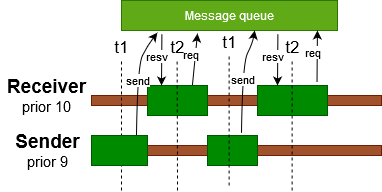
\includegraphics[width=0.7\columnwidth]{graphs/communication/signalblock.png}}
    \caption{Send unblock}
    \label{fig:signal_unblock}
    \vspace{-1.5em}
\end{figure}


While measuring message queues we also added 3 complex tests. The signal unblock scenario can be see in Figure \ref{fig:signal_unblock}. In this test we were measuring the context switch with sending a message to a message queue. The median time reached 528~ns, if we subtract the context switch time we get 360~ns. That is the corresponding time to send the message to the queue. The value is greater than a pure send because in this case we must include the blocking time because the queue might be full. By looking at the receive block, the situation is similar but with receive and we get the median of 863~ns. That is because of the blocking time as it tries to read the value for some time if there is no value.

The last complex test with message queues is a workload test. In this scenario we had also sender, receiver and another tasks with lower priority that were doing some work. Here, we were measuring the time to send the message but at the beginning of sender activity we set a delay so the lower priority task could be executed. The interesting part is in Figure \ref{fig:mq_stacked} where we can see in what percentage of our measurement is translated to context switch. It is both expected and obvious that in the maximum values, workload would require more time than context switching. In general we achieved much better results, compared to previous work \cite{b7, b5}, needing almost 10\% less cycles throughout the test.


% \begin{figure}[htbp]
%     \centerline{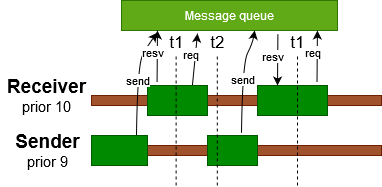
\includegraphics[width=0.7\columnwidth]{graphs/communication/receiveblock.png}}
%     \caption{Receive block}
%     \label{fig:signal_unblock}
% \end{figure}


% \vspace{-0.50mm}


\vspace{-5.00mm}
\begin{figure}[!htbp]
    \centerline{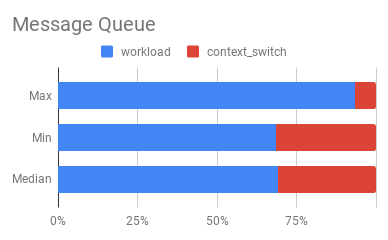
\includegraphics[width=0.7\columnwidth]{graphs/rpi/Message_Queue_stacked_3.png}}
    \caption{Message passing - workload analysis}
    \label{fig:mq_stacked}
\end{figure}

We can observe similar behavior with other tests also \textit{e.g. semaphores, mutexes, etc}.

Regarding semaphores we can see that results are coherent with message queue results, which is expected since both tests operate under the same principle. As we can see freeRTOS takes twice as much cycles to take and block a semaphore than to signal and switch a new task.

In mutexes tests we can notice the average is very close to the minimum values. This shows us that maximum values are not expected and are probably caused rarely by "extreme" cases. 
% We can also note that acquiring a mutex takes less time than releasing it. This is due to the many security checks performed before locking the mutex, while releasing takes the ownership for granted.

Comparing mutexes and semaphores, \textif{sem signal \& mutex acquisition} and \textif{sem wait \& mutex release} we can see that mutexes are slower which is rational. This is due to the many security checks performed by mutexes before locking or unlocking.

% \begin{figure}[htbp]
%     \centerline{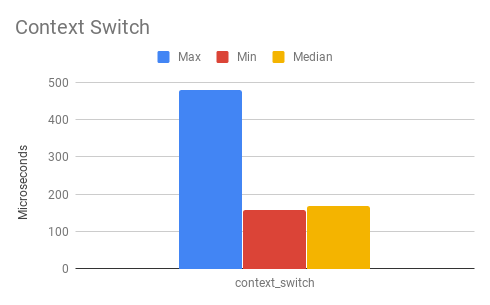
\includegraphics[width=0.7\columnwidth]{rpi/Context Switch.png}}
%     \caption{RPi 2B Hardware Setup.}
%     \label{demo}
% \end{figure}
% \begin{figure}[htbp]
%     \centerline{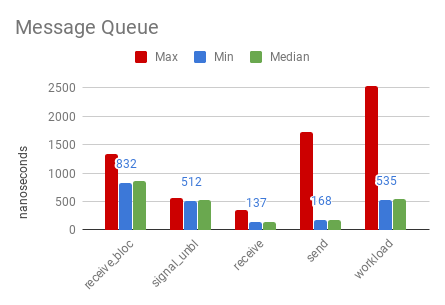
\includegraphics[width=0.7\columnwidth]{graphs/rpi/Message Queue.png}}
%     \caption{RPi 2B Hardware Setup.}
%     \label{mq_times}
% \end{figure}
% \vspace{-8.50mm} 

\begin{table}[htbp]
\begin{center}
\begin{tabular}{|l|c|c|c|}
\hline
\textbf{Name}           & \multicolumn{1}{l|}{\textbf{Min [ns]}} & \multicolumn{1}{l|}{\textbf{Median [ns]}} & \multicolumn{1}{l|}{\textbf{Max [ns]}} \\ \hline
mq context switch       & 157                                    & 168                                       & 480                                    \\ \hline
mq send                 & 168                                    & 182                                       & 1719                                   \\ \hline
mq receive              & \cellcolor[HTML]{C3D3D5}137            & \cellcolor[HTML]{C3D3D5}137               & 342,5                                  \\ \hline
mq send unblock       & 512                                    & 528                                       & 563                                    \\ \hline
mq receive block        & 832                                    & \cellcolor[HTML]{C3D3D5} 863               & 1337                                   \\ \hline
mq workload             & 535                                    & 544                                       & \cellcolor[HTML]{C3D3D5}2526           \\ \hline
mutex release unblock   & 518                                    & 529                                       & 1009                                   \\ \hline
mutex request block     & 1032                                   & 1056                                      & 1496                                   \\ \hline
mutex pip               & 1026           & 1042              & 1495                                   \\ \hline
mutex workload          & 528                                    & 529                                       & 780                                    \\ \hline
mutex acquisition       & 119                                    & 132               & 943                                    \\ \hline
mutex release           & 157                                    & 160                                       & 526                                    \\ \hline

sem signal unblock      & 420                                    & 427                                       & 448                                    \\ \hline
sem wait block          & 848                                    & 862                                       & 1393                                   \\ \hline
sem signaling with prio & 214                                    & 229                                       & 606                                    \\ \hline
sem signal              & 121                                    & 125                                       & 1352,5                                 \\ \hline
sem wait                & 100                                    & 100                                       & 289,5                                  \\ \hline
sem workload                & 698                                    & 698                                       & 2335                                 \\ \hline
\end{tabular}
\end{center}
    \label{tab:results}
    \caption{Results measured on Raspberry}
    \vspace{-1em}
\end{table}

\vspace{-4.00mm}

\section{Conclusion}

The advanced real-time systems will possess
capabilities for high-speed data processing and
communication which will require very high time
bound processing than what is available in state-of
the-art systems. This necessitates the need of
improving the real-time mechanisms in RTOS for our
future need. As proved in this report, freeRTOS might 
have room for improvement. To cope with  these 
challenges, very high  performance is necessary at all levels of
implementation application level and system level. 
The results show that real time operating system have better response
time compared to the general purpose operating system. 
In this paper we reviewed several Benchmarking
techniques for measuring the performance of RTOS
using real-time parameters. It is hoped that by
providing insights into the Benchmarking techniques,
this paper would help the researches in addressing the
implementation challenges of RTOS for efficient realtime systems of tomorrow.
\subsection{Video}

Short video presentation of our work: \url{https://www.youtube.com/watch?v=iywyAUN0roM}

\subsection{Members Contribution}
Each member contributed equally into the making of this report. (50\% - 50\%)

\vspace{-1.30mm}
\begin{thebibliography}{00}

\bibitem{b1} Wei-Tsun Sun; Zoran Salcic; , "Modeling RTOS for Reactive Embedded Systems," VLSI Design, 2007. doi:10.1109/VLSID.2007.111
\bibitem{b2} Yodaiken, Victor \& Barabanov, Michael. (2000). A real-time Linux.
\bibitem{b4} Weiderman, N.H., Kamenoff, N.I. Hartstone Uniprocessor Benchmark: Definitions and experiments for real-time systems. Real-Time Syst 4, 353–382 (1992).
\bibitem{b5} RTOS Benchmarking tests, Guillaume Champagne, \\ 
https://github.com/gchamp20/RTOSBench.
\bibitem{b6} FreeRTOS Scheduling, \\ 
https://www.freertos.org/implementation/a00005.html.
\bibitem{b7} Benchmarking Real Time Operating Systems, Guillaume Champagne, \\
Michel Dagenais, May 6, 2019, \\ https://amdls.dorsal.polymtl.ca/system/files/RTOS\%20\%20Benchmarking.pdf

\end{thebibliography}
\vspace{12pt}


\end{document}
